\documentclass[9pt,twocolumn,twoside]{Gunadarma}
\setboolean{shortarticle}{false}


\title{\begin{center}
		Pengembangan Aplikasi Pembayaran Online \textit{Mobile Money System} Dengan Menggunakan \textit{Agile} Metodologi
dan Teknologi \textit{Service Oriented Architecture}   
	\end{center}}

\author[1]{Candra Gunawan}
\affil[1]{Magister Manajement Sistem Informasi, Universitas Gunadarma, 2016, Jakarta}

\affil[*]{Corresponding author: sherard@outlook.com}

\dates{Compiled using \LaTeX\ \today}


\ociscodes{}

\doi{\url{http://Gunadarma.ac.id}}

\begin{abstract}
\textit{Mobile Money System} adalah suatu aplikasi bisa digunakan untuk berbagai macam pembayaran, mulai dari pembelian pulsa maupun belanja online. Dalam pengembangan aplikasi tersebut, dibutuhkan suatu metode pengembangan sistem yang bisa menjawab kebutuhan pasar yang sangat cepat. Dan juga, dibutuhkan suatu teknologi yang bisa beradaptasi dengan metode pengembangan sistem tersebut.
\textit{\textbf{Agile Development Methods}} adalah sekelompok metodologi pengembangan perangkat lunak yang di dasarkan pada prinsip - prinsip jangka pendek yang memerlukan adaptasi cepat dari pengembang terhadap perubahan dalam bentuk apapunrc. 
\textbf{\textit{service oriented architecture (SOA}} adalah suatu gaya arsitektur sistem yang membuat dan menggunakan proses bisnis dalam bentuk paket layanan sepanjang siklus hidup nya.
Dalam hal ini, akan dibahas bagaimana implementasi perancangan sistem pembayaran online dengan menggunakan metodologi \textit{agile} dan teknologi \textbf{\textit{SOA}}


\end{abstract}

\setboolean{displaycopyright}{true}

\begin{document}

\maketitle
\thispagestyle{fancy}
\ifthenelse{\boolean{shortarticle}}{\abscontent}{}

\section{Pendahuluan}
\subsection{Latar Belakang Masalah}
\textit{Mobile Money System} adalah salah satu alat pembayaran dengan menggunakan telepon genggam \textit{(handphone)}, atau disebut juga \textit{mobile money}. \textit{Mobile Money System} ini memungkinkan seseorang melakukan pembayaran suatu layanan dengan menggunakan \textit{handphone}, sehingga lebih mudah dan bisa dimana saja. 
untuk mengatasi kebutuhan pasar terhadap layanan pembayaran yang sangat cepat, maka penyediaan layanan tersebut harus di dukung dengan kemampuan dari sistem yang cepat ber-adaptasi dan cepat menyediakan kebutuhan pasar. 

Menyadari akan hal tersebut, maka diperlukan suatu metodologi yang bisa cepat ber-adaptasi terhadap kebutuhan pasar, dan bisa mendefinisikan pengembangan suatu layanan dengan cepat. Terkait dengan kebutuhan tersebut, maka pilihan nya adalah menggunakan \textbf{\textit{Agile Development Methodology}}, dibandingkan dengan menggunakan metodologi tradisional, seperti misalnya adalah \textbf{\textit{waterfall}}. 

Selain \textbf{\textit{Development Methodology}}, diperlukan juga suatu teknologi yang mendukung hal tersebut. Dimana teknologi tersebut membuat sistem bisa dikembangkan secara modular / \textit{service}. Sehingga modul - modul tersebut bisa di kembangkan secara terpisah dan bisa di \textit{re-use}. Karena itu maka di putuskan teknologi yang tepat adalah menggunakan \textit{\textbf{Service Oriented Architecture (SOA)}}. 


\subsection{Rumusan Masalah}
Rumusan masalah pada jurnal \textbf{"Pengembangan Aplikasi Pembayaran Online \textit{Mobile Money System} Dengan Menggunakan \textit{Agile} Metodologi"} adalah untuk menjelasakan bagaimana pengembangan sistem tersebut menggunakan \textbf{\textit{Agile Development Methodology}} dan dengan menggunakan \textbf{\textit{Service Oriented Architecture}} teknologi. 


\subsection{Tujuan Penulisan}
Tujuan penulisan ini adalah untuk menjelaskan peran \textbf{\textit{Agile Methodology}} dan tenologi \textbf{\textit{Service Oriented Architecture}} dalam menjawab kebutuhan permintaan pengembangan sistem yang cepat beradaptasi. 


\section{Landasan Teori}
\subsection{Agile Development Method}
\textbf{\textit{Agile Development Methods}} adalah sekelompok metodologi pengembangan perangkat lunak yang didasarkan pada prinsip-prinsip yang sama atau pengembangan sistem jangka pendek yang memerlukan adaptasi cepat dari pengembang terhadap perubahan dalam bentuk apapun. Agile development methods merupakan salah satu dari Metodologi pengembangan perangkat lunak yang digunakan dalam pengembangan perangkat lunak. Agile memiliki pengertian bersifat cepat, ringan, bebas bergerak, dan waspada. Sehingga saat membuat perangkat lunak dengan menggunakan agile development methods diperlukan inovasi dan responsibiliti yang baik antara tim pengembang dan klien agar kualitas dari perangkat lunak yang dihasilkan bagus dan kelincahan dari tim seimbang.

\begin{figure}[htbp]
\begin{center}
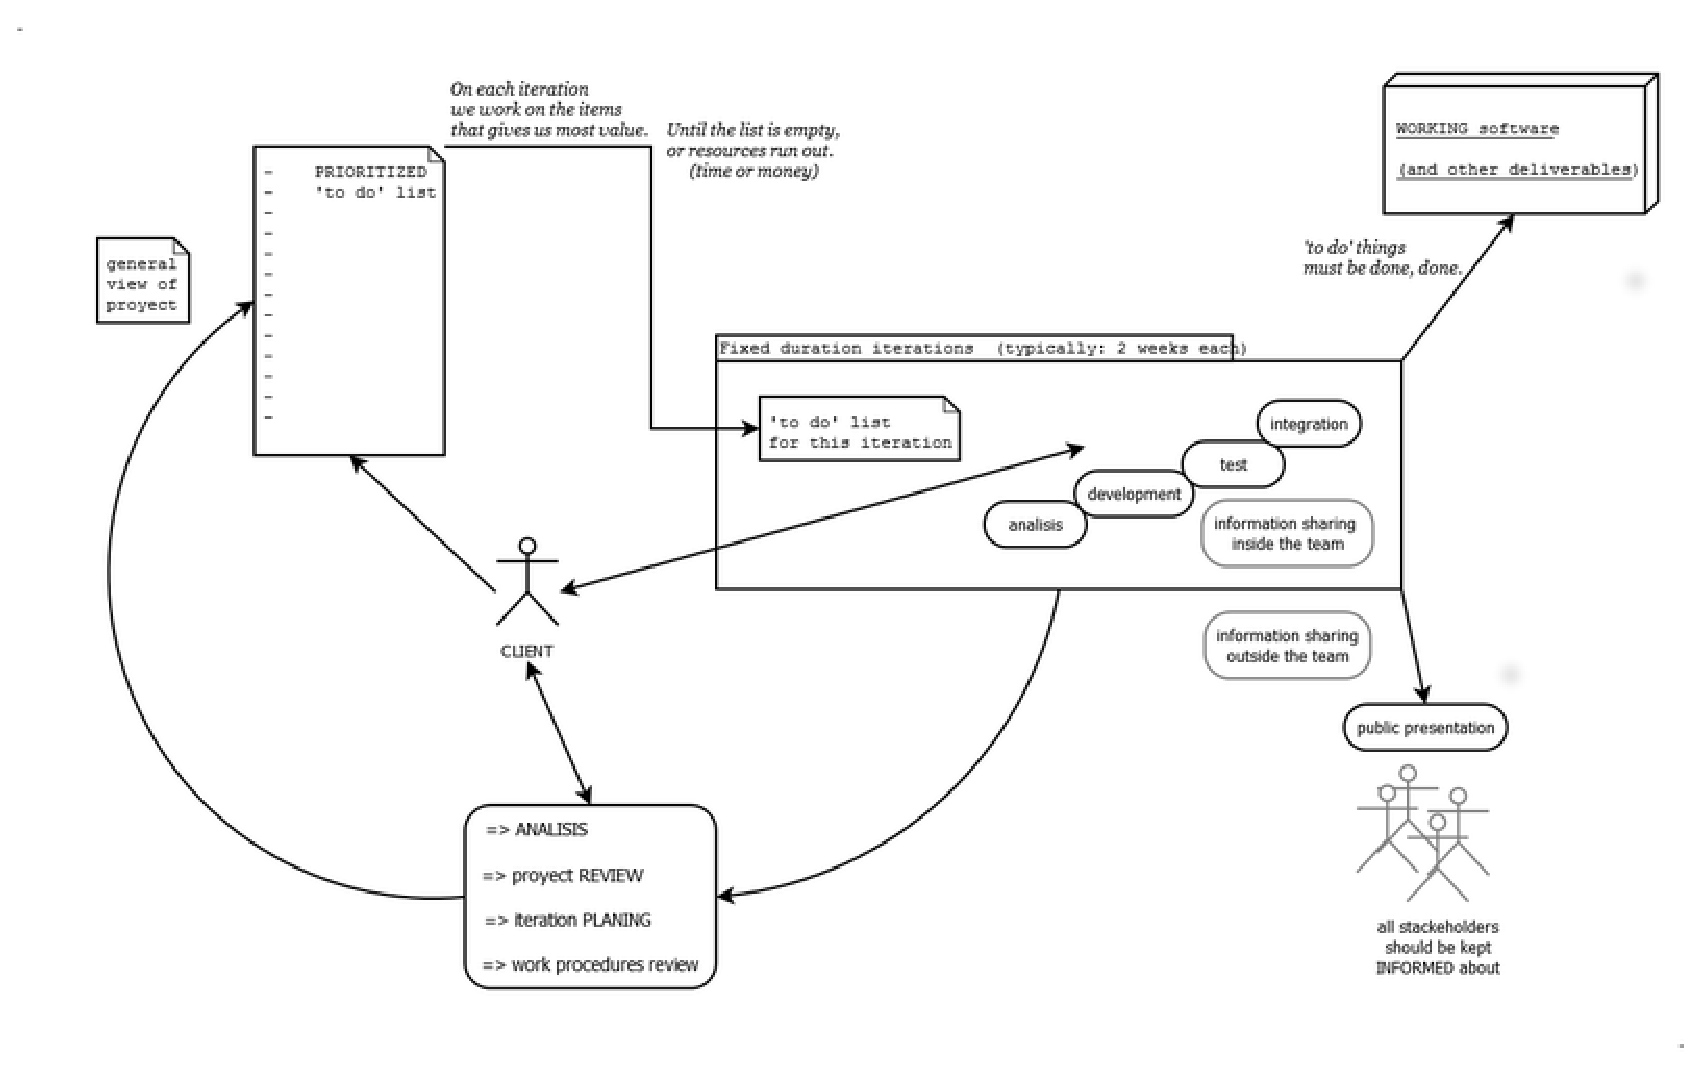
\includegraphics[width=1\columnwidth]{agile_methodology_for_software_development.eps} \label{fig:1-noFCase1}
\end{center}
\caption{Agile Methodology}
\end{figure}

Agile development methods terdefinisi dalam empat nilai, biasa di sebut \textbf{\textit{Agile Alliance’s Manifesto}}. Berikut ini isi dari \textbf{\textit{Agile Alliance’s Manifesto \cite{Agile:01}}} : 

\begin{center}
{\Large \textbf{\textit{Manifesto for Agile Software Development}}}
\end{center}

\textbf{We are uncovering better ways of developing
software by doing it and helping others do it.
Through this work we have come to value:}
\\

\textbf{\Large{Individuals and interactions}}over processes and tools

\textbf{\Large{Working software}} over comprehensive documentation

\textbf{\Large{Customer collaboration}} over contract negotiation

\textbf{\Large{Responding to change over}} following a plan
\\

\textbf{That is, while there is value in the items on
the right, we value the items on the left more.}
\\

Dari \textbf{\textit{Agile Manifesto}} terdefinisi dalam empat nilai :
\begin{itemize}
\item \textbf{Interaksi dan personel} lebih penting daripada proses dan alat.
\item \textbf{Perangkat lunak yang berfungsi} lebih penting daripada dokumentasi yang lengkap.
\item \textbf{Kolaborasi dengan klien} lebih penting daripada negosiasi kontrak.
\item \textbf{Respon terhadap perubahan} lebih penting daripada mengikuti rencana.
\end{itemize}

\subsection{Service Oriented Architecture}

\textbf{SOA (service oriented architecture}, arsitektur berorientasi layanan) adalah suatu gaya arsitektur sistem yang membuat dan menggunakan proses bisnis dalam bentuk paket layanan sepanjang siklus hidupnya. SOA membagi fungsi - fungsi menjadi unit - unit yang berbeda (layanan), yang dapat di distribusikan melalui suatu jaringan dan dikombinasikan serta digunakan ulang untuk membentuk aplikasi bisnis.


\begin{figure}[htbp]
\begin{center}
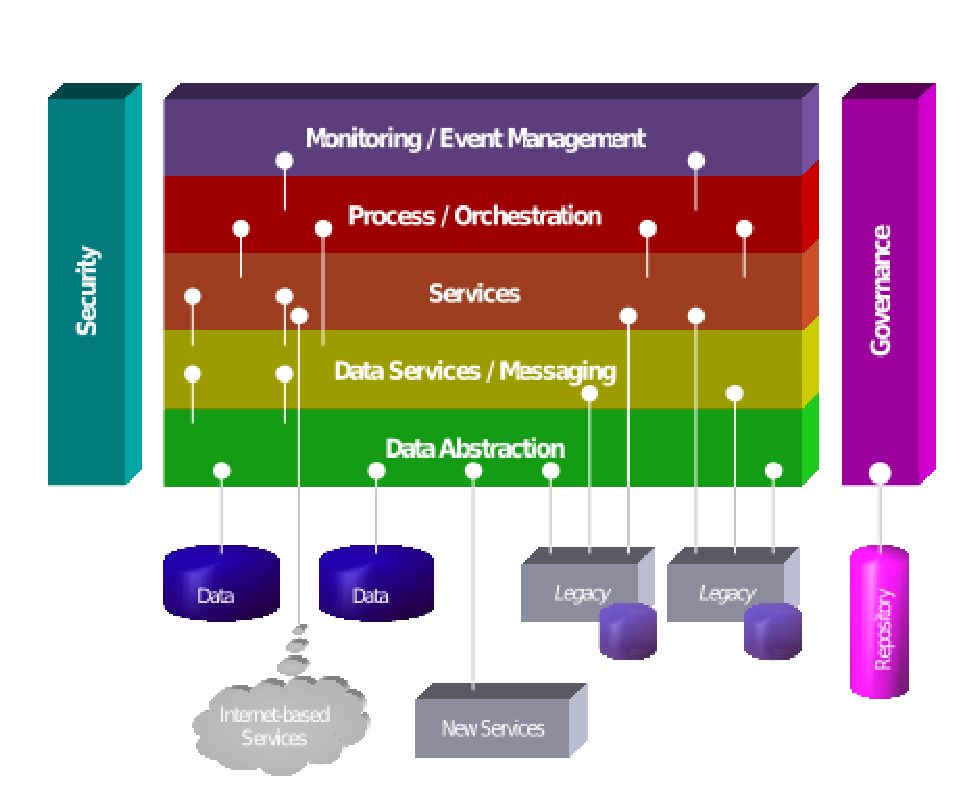
\includegraphics[width=1\columnwidth]{SOA_Metamodel.eps} \label{fig:3-noFCase1}
\end{center}
\caption{SOA Model}
\end{figure}

Dalam meng-implementasikan \textit{service-oriented architecture}, bisa menggunakan web service \textit{( Web Service Approach )}. Yaitu dengan membuat fungsi - fungsi yang independent dan bisa di akses melalui jaringan, dan tidak tergantung kepada \textit{platform} dan bahasa pemrograman. Service ini bisa me-representasikan suatu aplikasi atau sebagai \textit{wrapper} suatu \textit{legacy system} agar bisa di akses melalui jaringan. 

Setiap aplikasi SOA bisa mempunyai role seperti berikut ini :
\begin{enumerate}
\item \textit{Service provider}. Merupakan aplikasi yang menyediakan web service. Setiap service provider harus menyediakan service - service yang bisa di gunakan dalam bentuk \textit{interface}. 
\item \textit{Service consumer}. Yaitu aplikasi yang akan menggunakan service tersebut (\textit{consume}). 
\end{enumerate}

Dalam implementasi nya, dalam membangun SOA menggunakan standar komunikasi \textit{web service} seperti misalnya menggunakan SOAP (\textit{Simple Object Access Protocol}). Tetapi bisa juga menggunakan metode komunikasi lain yang di sepakati. 


\section{Pembahasan}

\subsection{Service Pembayaran Online}
Dalam Bab ini, penulis akan menggambarkan service yang dibuat. Dengan asumsi beberapa service sudah tersedia sebelum nya, maka disini hanya akan di batasi kepada service utama nya. Juga pembahasan akan dibatasi hanya pada spesifikasi service tersebut, tapi tidak ke implementasi nya. Berikut ini design service yang terlibat / yang akan dibuat dalam penulisan berikut ini :
\begin{figure}[htbp]
\begin{center}
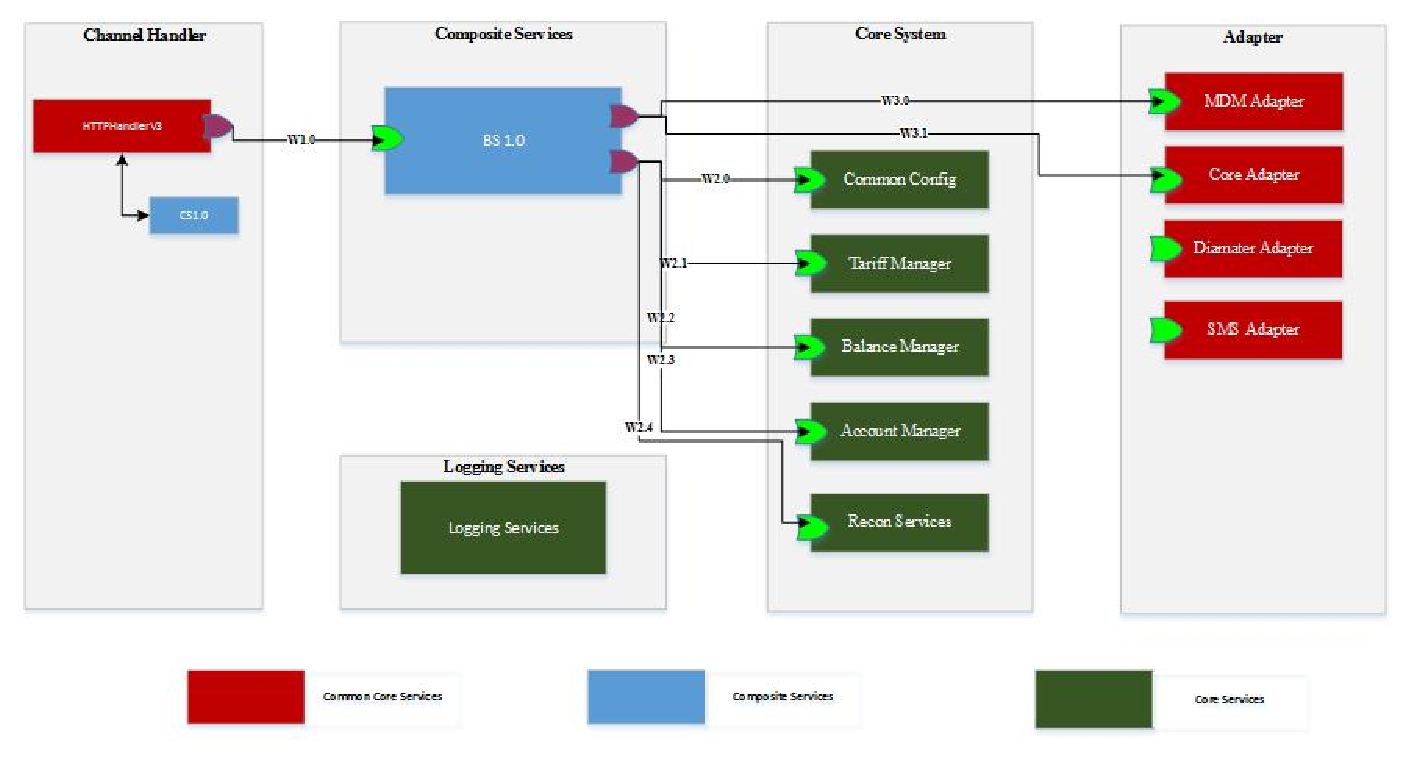
\includegraphics[width=1\columnwidth]{BuildingBlockDiagram.eps} \label{fig:3-noFCase1}
\end{center}
\caption{Service Model}
\end{figure}
 
service yang akan dibuat adalah :
\begin{table}[htbp]
\centering
\small
\caption{\bf Daftar Service}
\scalebox{0.8}{
\begin{tabular}{|c|c|c|c|}
\hline No & Service Code & Service Category &  Service Name \\
\hline 1 & BS1.0 & Business services & svgBilXLTunaiPartnerServicesV1.0 \\
\hline
\end{tabular}
}
  \label{tab:Daftar Service}
\end{table}
\\
\\
untuk spesifikasi interface service adalah seperti berikut ini :
\begin{table}[htbp]
\centering
\small
\caption{\bf Daftar Interface}
\scalebox{0.7}{
\begin{tabular}{|c|c|c|c|c|}
\hline Wire Code & Call Method & Service Consumer &  Service Provider & Operation Name \\
\hline W2.0 & SOAP & BS1.0 & Common Config & OpGetConfig \\
\hline W2.1 & SOAP & BS1.0 & Tariff Manager & opGetTariffAmount \\
\hline W2.2 & JMS & BS1.0 & Balance Manager & opAdjustBalance \\
\hline W2.2 & JMS & BS1.0 & Account Manager & opGetCustomerData \\
\hline W2.2 & JMS & BS1.0 & Account Manager & opGetMerchantData \\
\hline
\end{tabular}
}
  \label{tab:Daftar Interface}
\end{table}

\subsection{Business Process Model}
Berikut ini Business Process Model untuk menggambarkan design dari aplikasi. 
\begin{figure}[htbp]
\begin{center}
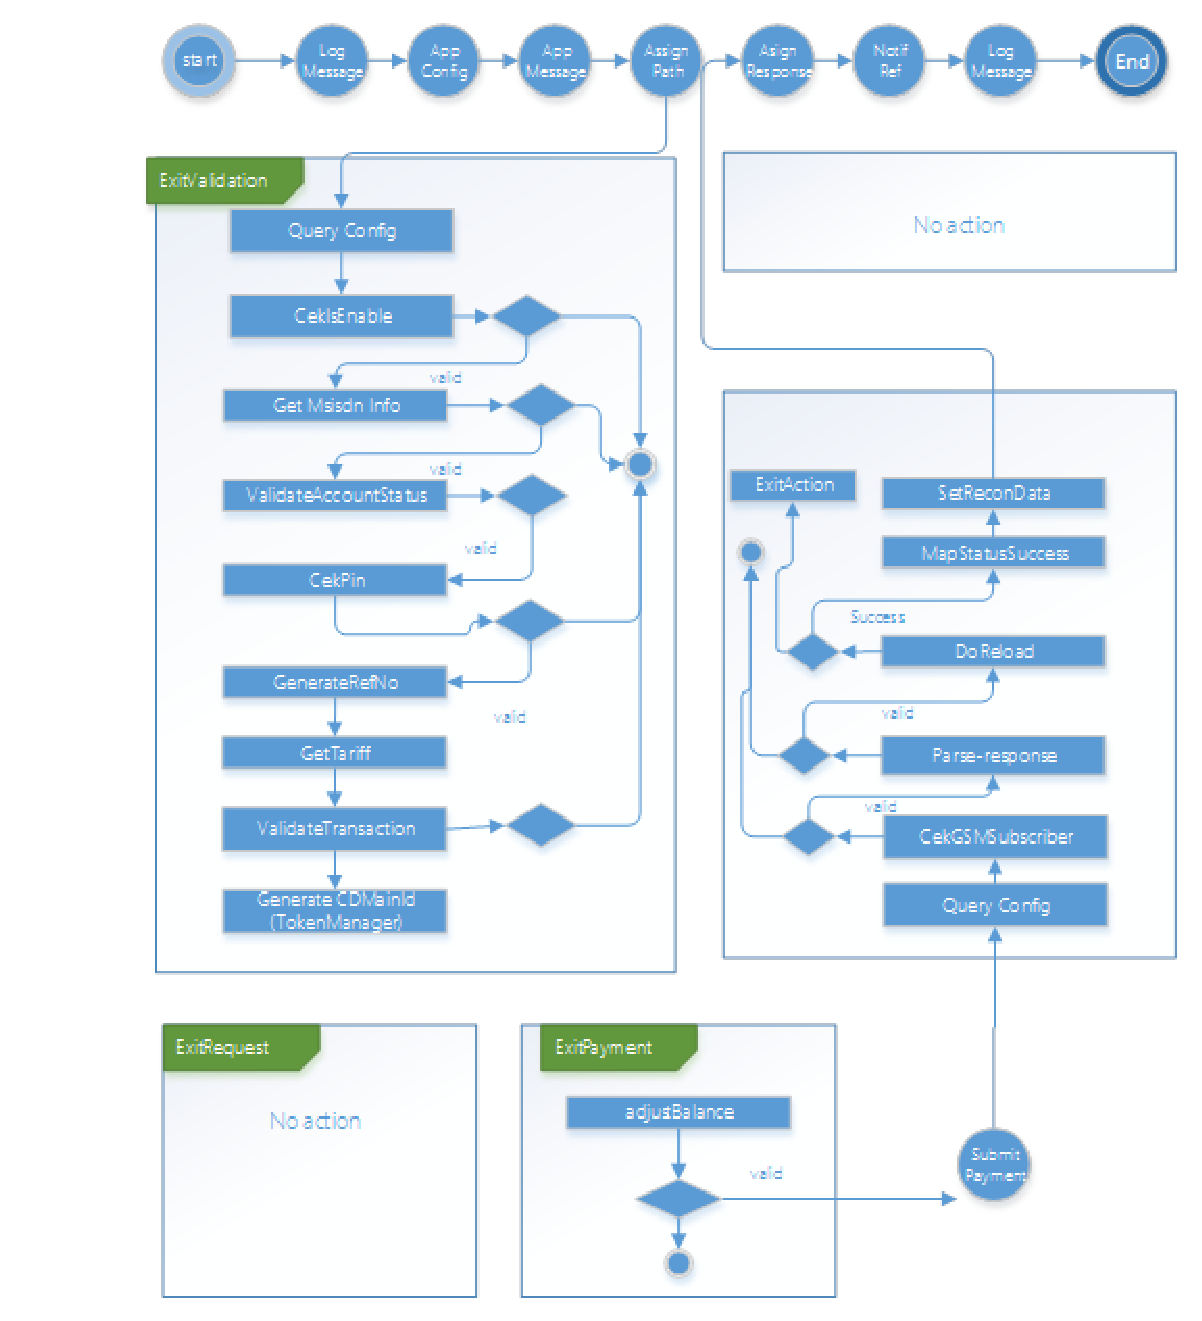
\includegraphics[width=1\columnwidth]{BusinessFlow-1.eps} \label{fig:3-noFCase1}
\end{center}
\caption{Business Flow}
\end{figure}
\\ \\ \\ \\ \\ \\ \\ \\ \\ \\ \\ \\ \\ \\ \\ \\ \\ \\ \\ \\ 
\\ \\ \\ \\ \\ \\ \\ \\ \\ \\ \\ 

\subsection{Skema XML}
Berikut ini skema XML yang digunakan dalam service ini :
\begin{table}[htbp]
\centering
\small
\caption{\bf Skema \textit{Payment}}
\scalebox{0.9}{
\begin{tabular}{|c|c|c|c|}
\hline Payload Name & Sub element Name & Data Type &  Mandatory \\
\hline PaymentRq & PaymentRq & Complex Element & Optional  \\
\hline PaymentRq & MSISDN & String & N  \\
\hline   & service-id & String & N  \\
\hline   & order-id & String & N  \\
\hline   & Reference-no & String & N  \\
\hline   & amount & String & N  \\
\hline   & RequestPayload & Complex Element, Any & N  \\

\hline
\end{tabular}
}
  \label{tab:Skema Payment}
\end{table}


\subsection{Agile}
Pada tahap ini, penulis mencoba untuk membuat implementasi dari \textit{agile methodology}. Dalam melaksanan proses \textit{agile} ini, ada beberapa \textit{term} yang harus di mengerti :
\begin{itemize}
\item \textit{Iteration}. Adalah periode dimana \textit{agile} tim harus menyelasikan tugas yang sudah di sepakati di awal. Dalam hal ini adalah mengembangkan aplikasi yang sudah di definisikan bersama. Setelah proses ini selesai, maka tim harus siap untuk me-respon perubahan dan adaptasi terhadap pengembangan aplikasi.
\item \textit{Task}. Adalah list pekerjaan yang sudah di detailkan dalam mengembangkan aplikasi. Biasanya \textit{task} ini lebih kepada pembagian dari fungsi - fungsi dari aplikasi.
\item \textit{Backlog}. Adalah sekumpulan dari \textit{task} yang harus di kerjakan berikut nya oleh tim. \textit{Task} yang harus dikerjakan ini, bisa jadi adalah task yang belum selesai sebelum nya. 
\end{itemize}

Dalam pengembangan aplikasi ini, dilakukan \textit{project tracking} dengan menggunakan agile methodology. Pertama kali dalam agile methodology adalah dengan membuat \textit{story} dari aplikasi tersebut. 

\begin{figure}[htbp]
\begin{center}
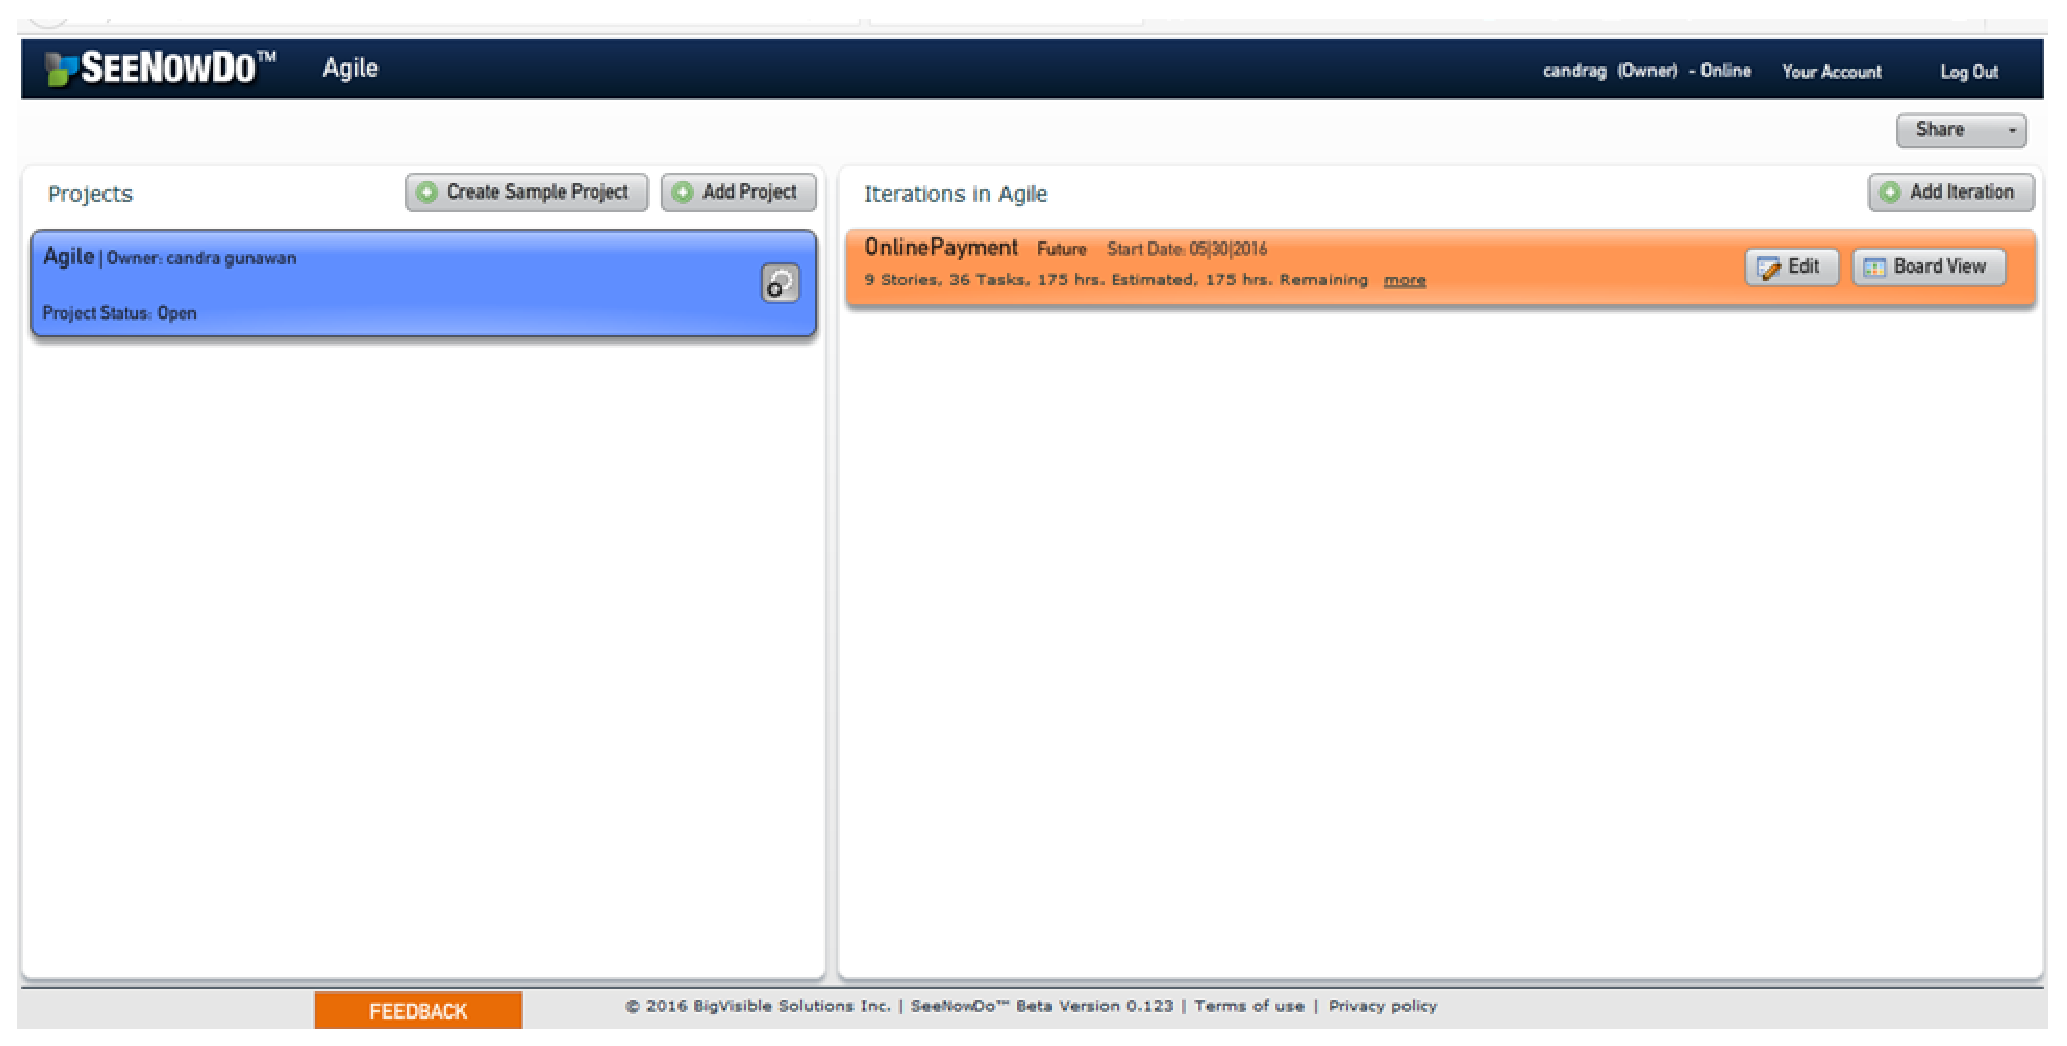
\includegraphics[width=1\columnwidth]{Agile-1.eps} \label{fig:3-noFCase1}
\end{center}
\caption{Agile Story}
\end{figure}

Setelah dibuat \textit{story} utama, maka bisa dibuat \textit{sub story} dalam pengembangan aplikasi tersebut.
\textit{Sub-story} tersebut dalam agile, dibuat menjadi task - task. Lalu di tracking tahapan nya. Dalam setiap \textit{task}, bisa secara \textit{independent} di lakukan, bisa \textit{on-progress}, \textit{backlog}, atau memang sudah ada yang \textit{done}. 

\begin{figure}[htbp]
\begin{center}
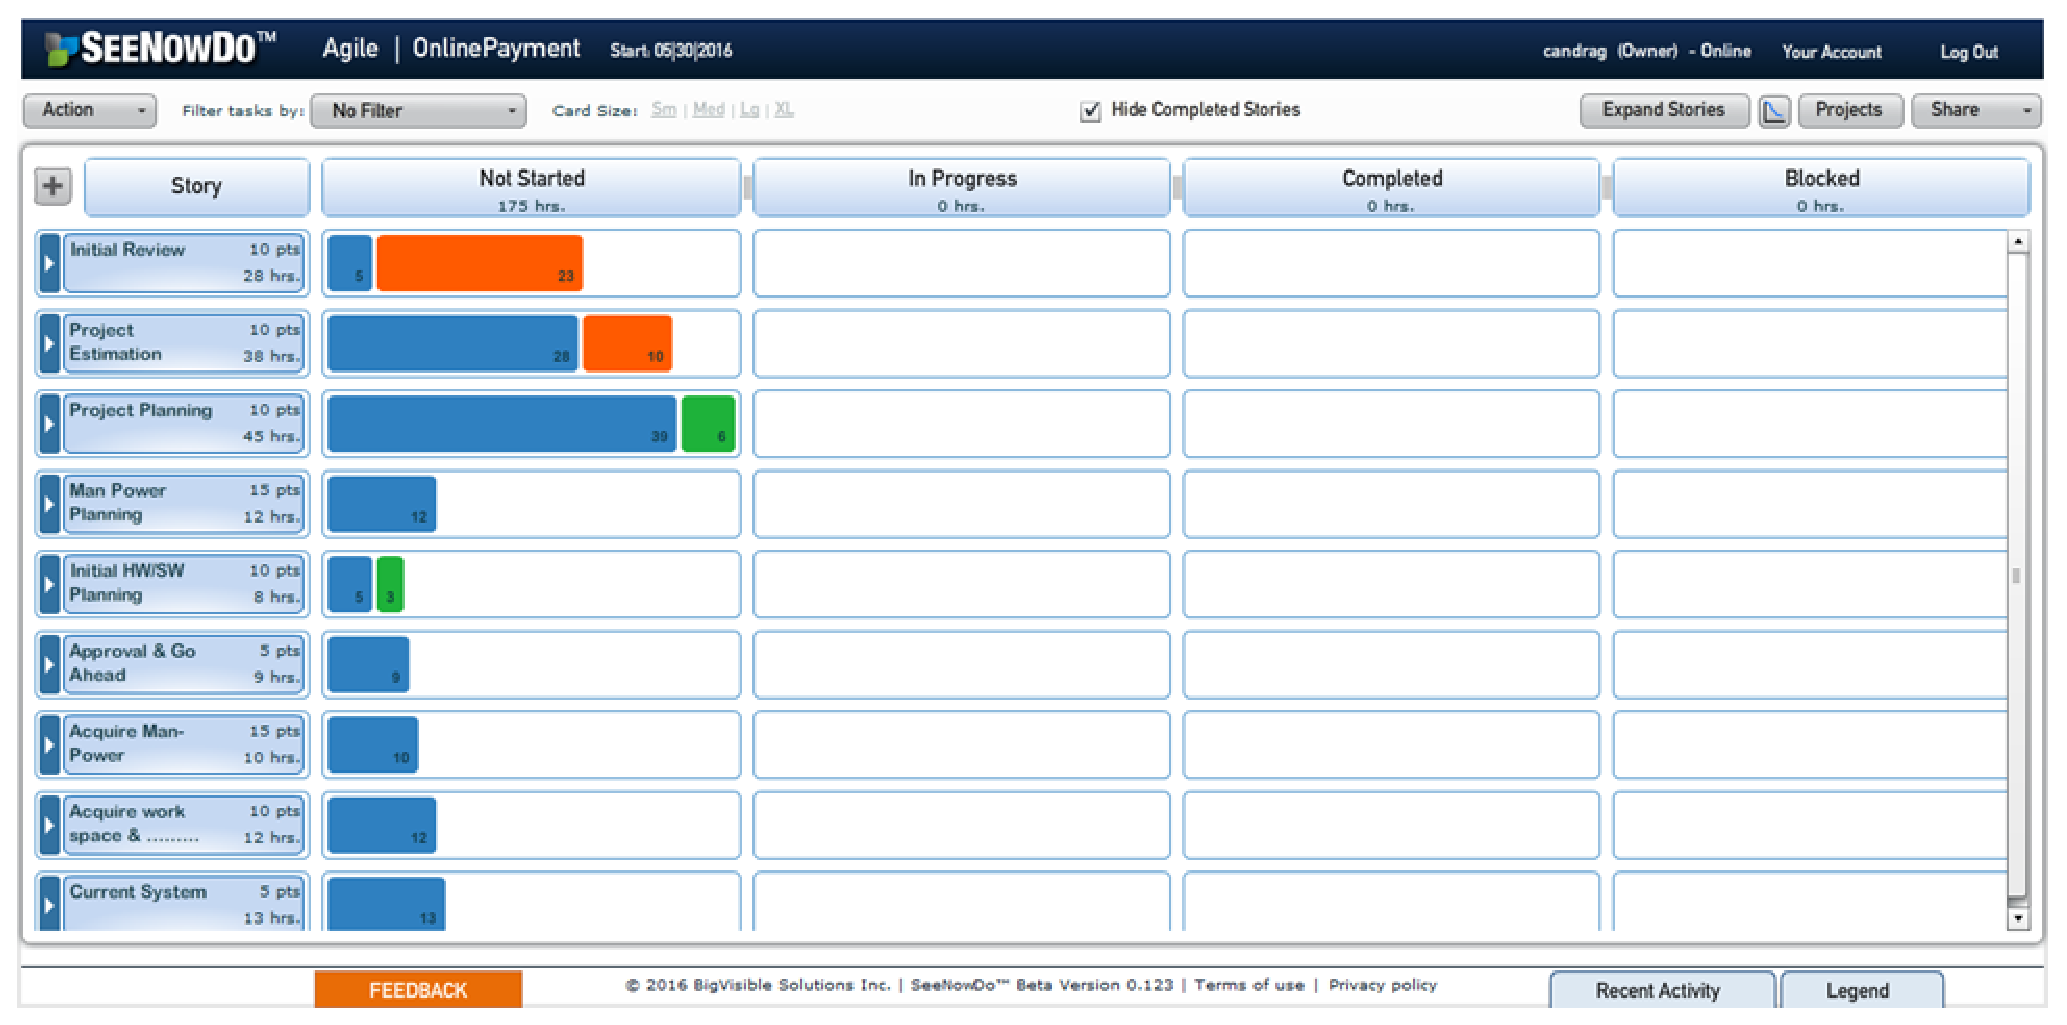
\includegraphics[width=1\columnwidth]{Agile-2.eps} \label{fig:3-noFCase1}
\end{center}
\caption{Agile Sub-Story}
\end{figure}

\begin{figure}[htbp]
\begin{center}
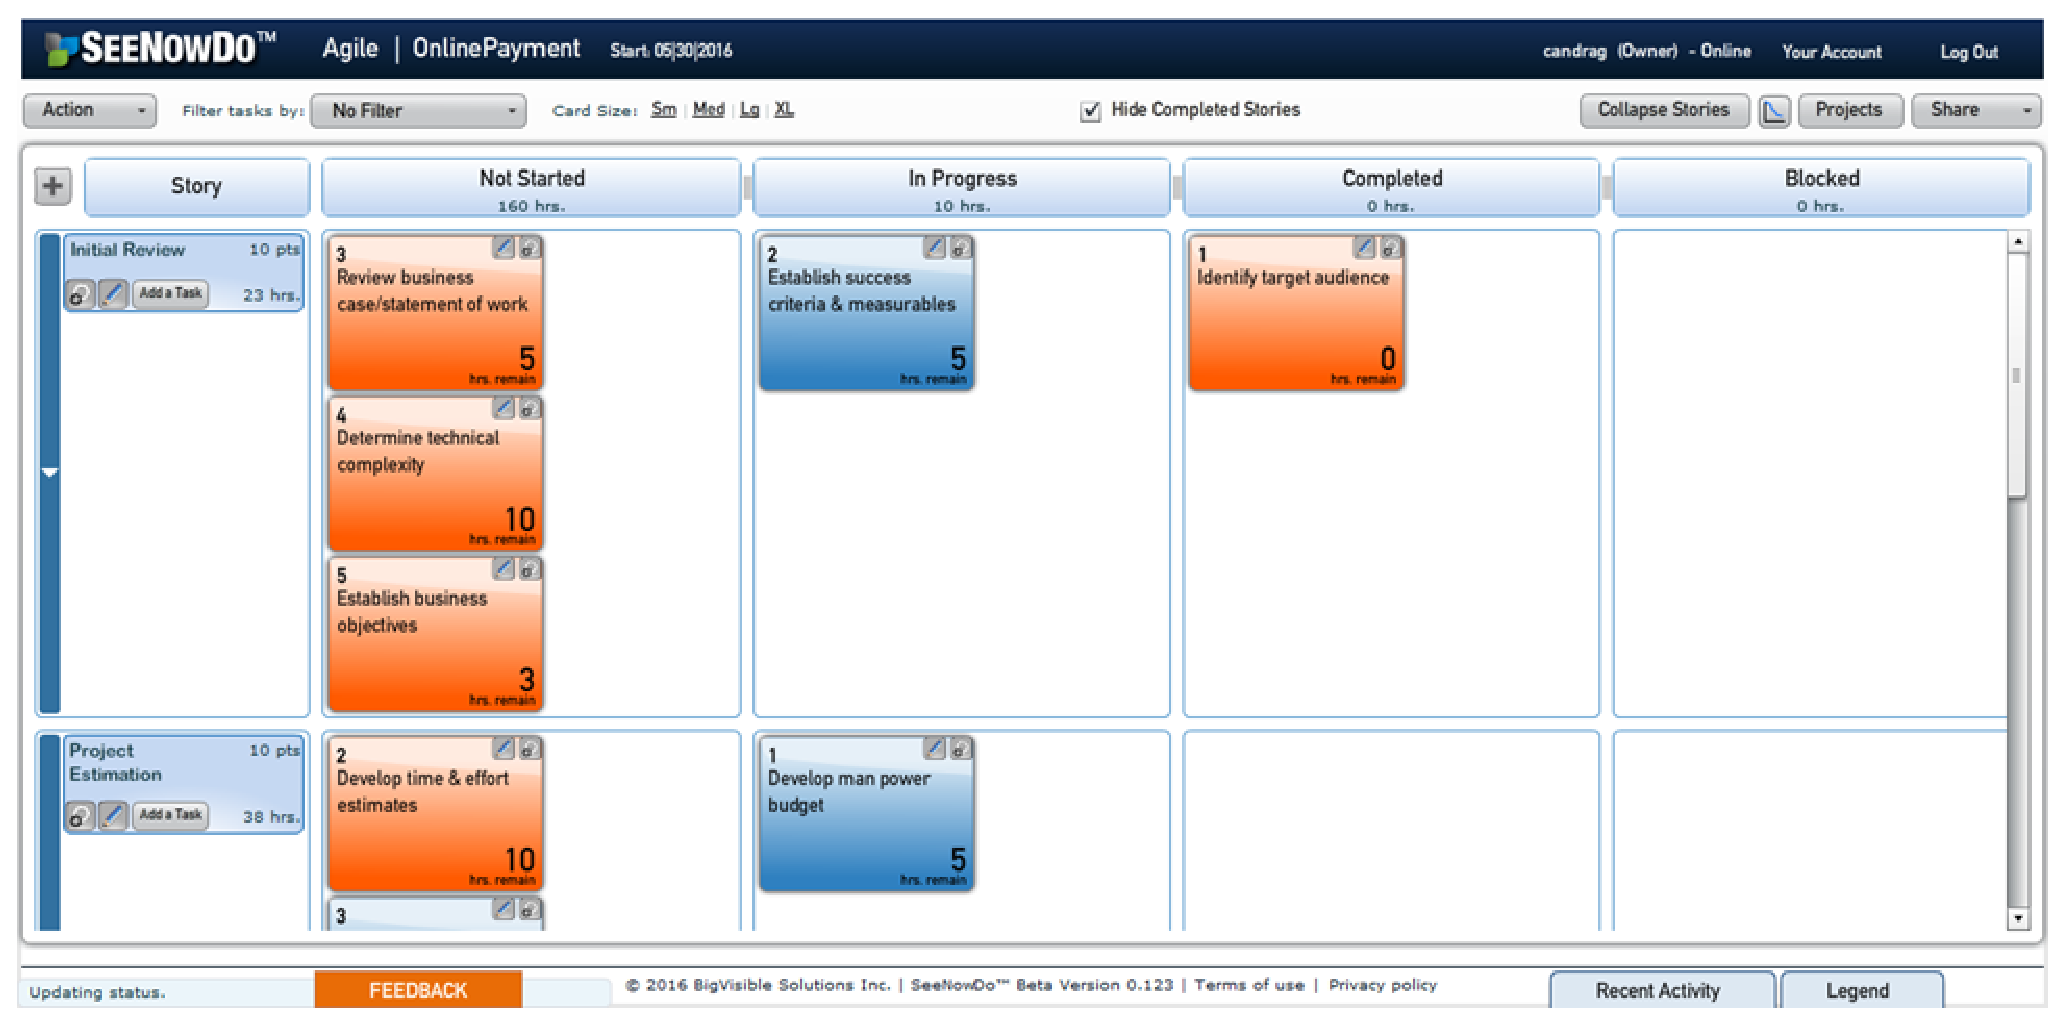
\includegraphics[width=1\columnwidth]{Agile-3.eps} \label{fig:3-noFCase1}
\end{center}
\caption{Agile Progress}
\end{figure}

Dengan melakukan pengembangan aplikasi dengan metode \textit{Agile}, setiap story dapat berjalan \textit{independent}, tetapi dengan tujuan yang sama. Dan juga, untuk suatu \textit{task}, bisa di \textit{tracking} secara independent. Proses penyelesaian aplikasi pun bisa lebih cepat, karena setiap task, harus bisa di \textit{deliver}. 

\section{Kesimpulan}
\subsection{Rangkuman}
\textit{Agile Methodology} memungkinkan proses pengembangan sistem dan aplikasi menjadi lebih cepat. Karena aplikasi akan di buat menjadi bentuk \textit{story - story} dan \textit{task} yang detail. Untuk proses \textit{delivery} setiap \textit{task} detail. Karena agar proses setiap \textit{task} bisa segera di evaluasi. Dan prinsip dari \textit{Agile} adalah me-respon perubahan, maka jika ada perubahan, bisa dikerjakan di \textit{task} atau \textit{story }berikut nya.

\textit{Service Oriented Architecture (SOA)} di \textit{implementasikan} disini untuk mendukung metodologi \textit{agile} ini. Sehingga apliksai bisa dibuat berdasarkan layanan, dan \textit{lousy coupled}. sehingga di harapkan tidak ada saling ketergantungan, dan setiap perubahan / adaptasi dilakukan tidak saling impact. 

\subsection{Saran}
Adapun dari penulisan berikut ini, ada beberapa saran yang penulis rangkum di dalam penulisan ini :
\begin{itemize}
\item Penulis baru menggambarkan perancangan sistem dengan menggunakan agile pada proses bisnis utama, dengan asumsi komponent lain sudah tersedia
\item Penulis menulisakan spesifikasi SOA dengan anotasi \textit{SCA (Service Composite Architecture)} dan baru di leve interface nya saja.
\ item Penulis belum melakukan menampilkan data komparasi antara metode biasa (contoh nya SDLC) dan dengan agile. Manakah yang lebih efisien. 
\end{itemize}

\section{Daftar Pustaka}


%\bigskip \noindent See \href{link}{Supplement 1} for supporting content.

%\noindent Add citations manually or use BibTeX. See \cite{Zhang:14}.
%\noindent Add citations manually or use BibTeX. See \cite{Agile:01}.
% Bibliography

\bibliography{sample}

%Manual citation list
%\begin{thebibliography}{1}
%\bibitem{Zhang:14}
%Y.~Zhang, S.~Qiao, L.~Sun, Q.~W. Shi, W.~Huang, %L.~Li, and Z.~Yang,
% \enquote{Photoinduced active terahertz metamaterials with nanostructured
%vanadium dioxide film deposited by sol-gel method,} Opt. Express \textbf{22},
%11070--11078 (2014).
%\end{thebibliography}

\end{document}